\section*{Examen del Molinos}

\subsection*{Foto de consigna}
\begin{figure}[H]
    \centering
    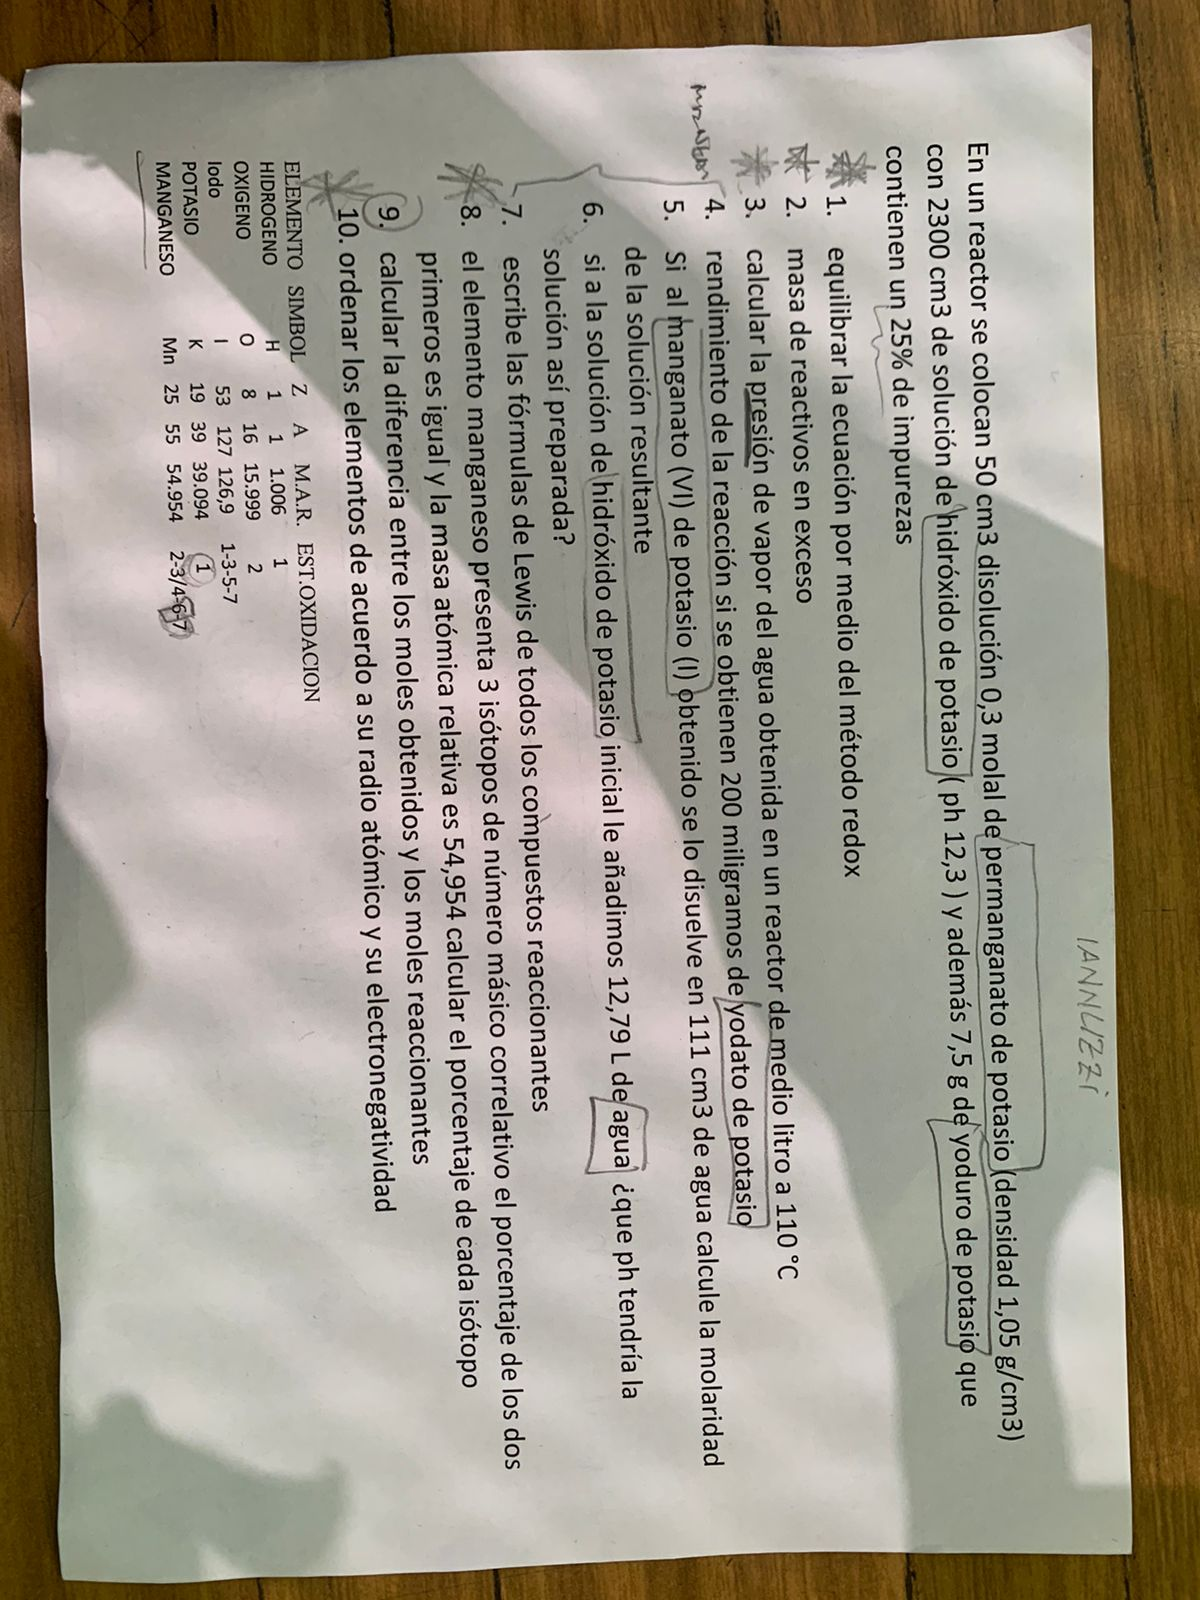
\includegraphics[width=0.7\linewidth, angle=90]{Images/molinos_examen1.jpg}
\end{figure}

\subsection*{Resolución}

\begin{enumerate}
\setlength\itemsep{2\baselineskip}

\item Balanceo por redox:
$$\ce{KMnO_4 + KOH + KI -> KIO_3 + K_2MnO_4}$$

Escribo los números de oxidación:
$$\ce{K^{+1}Mn^{+7}O_4^{-2} + K^{+1}O^{-2}H^{+1} + K^{+1}I^{-1} -> K^{+1}I^{+5}O_3^{-2} + K_2^{+1}Mn^{+6}O_4^{-2}}$$

Identifico cuál se oxida, cuál se reduce, al agente oxidante y al agente reductor:
\begin{table}[H]
    \centering
    \begin{tabular}{ll}
    Se oxida: & I \\
    Se reduce: & Mn \\
    Agente oxidante: & \ce{KMnO_4} \\
    Agente reductor: & \ce{KI}
    \end{tabular}
\end{table}

Identifico que es medio básico, planteo las semirreacciones, las balanceo e igualo los electrones:
\begin{multicols}{2}
    \underline{Semirreacción de oxidación:}
    $$\ce{I^- + 6OH^- ->
    IO_3^- + 3H_2O + 6e^-}$$
    
    \underline{Semirreacción de reducción:}
    $$\left( \ce{MnO_4^- + e^-  ->
    MnO_4^{2-}} \right) \cdot 6$$
\end{multicols}

Sumo las semirreacciones: 
$$\ce{
I^- + 6 OH^- + 6MnO_4 + \xcancel{6e^-} -> IO_3^- + 3H_2O + 6 MnO_4^{2-}\xcancel{6e^-}
}$$

Finalmente se ponen los coeficientes en la reacción original:
$$\fbox{\ce{6KMnO_4 + 6KOH + KI ->
KIO_3 + 6K_2MnO_4 + 3H_2O}}$$


\item Masa de reactivos en exceso:
$$\ce{6KMnO_4 + 6KOH + KI ->
KIO_3 + 6K_2MnO_4 + 3H_2O}$$

Calculo los moles de \ce{KMnO_4}:

\hfil$V_{\text{SC}}=50\text{cm}^3$
\hfil0,3m
\hfil$\delta = 1,05 \frac{\text{g}}{\text{cm}^3}$
\hfil $M = 158\frac{\text{g}}{\text{mol}}$

\hfil
Hay $2,37\text{g}\equiv 0,015 \text{mol}$ de $\ce{KMnO_4}$
\hfil

Calculo los moles de \ce{KOH}:

\hfil $V_{\text{SC}}=2,3 L$
\hfil pH = 12,3
\hfil 

\hfil
Hay $2,576\text{g} \equiv 0,046 \text{mol}$ de KOH
\hfil

Calculo los moles de \ce{KI}:

\hfil $m_i = 7,5g (\text{pureza}75\%)$
\hfil $M = 166\frac{\text{g}}{\text{mol}}$
\hfil

\hfil
Hay $5,625\text{g} \equiv 0,0339 \text{mol}$ de KI
\hfil

El limitante es \ce{KMnO_4}. Sobran 0,031 mol $\equiv$ 1,74g de KOH y 0,0314 mol $\equiv$ 5,21 g de KI.

Finalmente: 

\hfil
\fbox{masa de reactivos en exceso = 6,95 g}
\hfil


\item Presión del vapor del agua obtenida en un reactor de medio litro a 110ºC:
\begin{align*}
    P \cdot 0,5 \text{ l} &= 0,0075 \text{ mol} \cdot 0,082 \frac{\text{l}\cdot \text{atm}}{\text{mol} \cdot \text{K}} \cdot 383 \text{ K}\\
    P &= \dfrac{0,236 \text{ atm}}{0,5}\\
    \Aboxed{P &= 0,471\text{ atm}}
\end{align*}


\newpage
\item 0,2 g de \ce{KIO3} es $9,35\cdot 10^{-4}$ mol.

Con un rendimiento del \%100:
\rot{6}{1}{0,015}{2,5\cdot 10^{-3}}{mol de \ce{KMnO4}}{mol de \ce{KIO3}}

El rendimiento final es:

\hfil\fbox{
$\dfrac{9,35\cdot 10^{-4}}{2,5 \cdot 10^{-3}} \cdot 100\%
= 37,4\%$
}\hfil


\item Se obtienen $0,015\cdot 0,374 = 0,00561$ mol de \ce{K2MnO4}
\rot{0,00561}{0,111}{0,0505}{1}{mol}{l}
\hfil\fbox{
M = 0,0505
}
\hfil


\item 2,3 l de KOH, pH=12,3, le agrego 12,79 l de agua, calcular pH final.

\hfil $\text{pH}=12,4 \Rightarrow \text{pOH} = 1,7 \Rightarrow \left[\ce{OH^-}\right] = 10^{-1,7} = 0,02 $
\hfil
\rot{0,02}{1}
{0,046}{2,3}
{mol de \ce{OH^-}}{L}

Luego de diluir:
\rot{0,046}{15,09}
{3,05\cdot 10^{-3}}{1}
{mol de \ce{OH^-}}{L}

Finalmente:

\hfil \fbox{
$\text{pOH} = -\log\left( 3,05 \cdot 10^{-3} \right) = 2,52 \Rightarrow \text{pH} = 11,48$
}\hfil


\item xd

\item $A_1=53,\ A_2=54 y\ A_3=55.$
\begin{align*}
    53 \cdot p + 54 \cdot p + 55 \cdot (1 - 2p) &= 54,954\\    
    55 - 3p &= 54,954\\
    0,046 &= 3p\\
    p &= 0,0153
\end{align*}

Finalmente:

\hfil \fbox{
$p_1 = 1,53 \%,\ p_2 = 1,53 \%,\ p_3= 96,94 \%$
}\hfil


\item Sabiendo que reaccionan 0,015 mol de \ce{KMnO4}:

Moles obtenidos:

\hfil
0,015 mol \ce{K2MnO4} + 0,0075 mol de \ce{H2O} + 0,00375 mol de \ce{KIO3} = 0,02625 moles obtenidos
\hfil

Moles reaccionantes:

\hfil
0,015 mol \ce{KMnO4} + 0,015 mol de \ce{KOH} + 0,00375 mol de \ce{KI} = 0,03375 moles reaccionantes
\hfil


Finalmente:

\hfil \fbox{
$0,02625 - 0,03375 \text{ mol } = -0,0075\text{ mol}$
}\hfil


\item Radio atómico: H, O, K, Mn, I.
\hfil
Electronegatividad: K, Mn, H, I, O.
\hfil

\end{enumerate}

